\documentclass[unicode, 12pt, a4paper,oneside]{article}
\usepackage{booktabs}
\usepackage[utf8]{inputenc}
\usepackage[russian]{babel}
\usepackage{amsmath}
\usepackage{graphicx}
\begin{document}
    \title{Лабораторная работа №1\\Ларионов Даниил\\НФИбд-01-16}
    \maketitle
    \section{Уравнение движения}
    Уравнение, описывающее движение катера, с начальными условиями для двух случаев:
    $$\frac{x}{v} = \frac{k-x}{2.3v}$$
    $$\frac{x}{v} = \frac{k+x}{2.3v}$$
    Отсюда получаем $x_1 = k*0.30303, x_2=k*0.769231$. Находим скорости: $v_1 = \sqrt{5.29v^2-v^2} = \sqrt{4.29v^2}$.
    Тогда получаем 
    \begin{cases}
        $\frac{dr}{dt} = v$\\
        $r*\frac{d\theta}{dt} = \sqrt{4.69}*v$
    \end{cases}
    с начальными условиями
    \begin{cases}
        $\theta_0 = 0$\\
        $r_0 = x_1$
    \end{cases}
    и
    \begin{cases}
        $\theta_0 = -\pi$\\
        $r_0 = x_2$
    \end{cases}\\
    Исключаем производную по t и получаем:
    $$\frac{dr}{d\theta} = \frac{r}{\sqrt{4.69}}$$
    \section{Траектории движения катера и лодки для двух случаев}
    {\bf Первый случай} 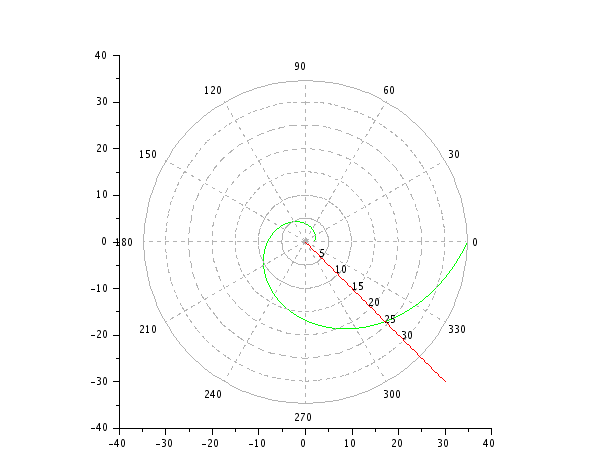
\includegraphics[width=\textwidth]{var1.png}\\
    {\bf Второй случай} 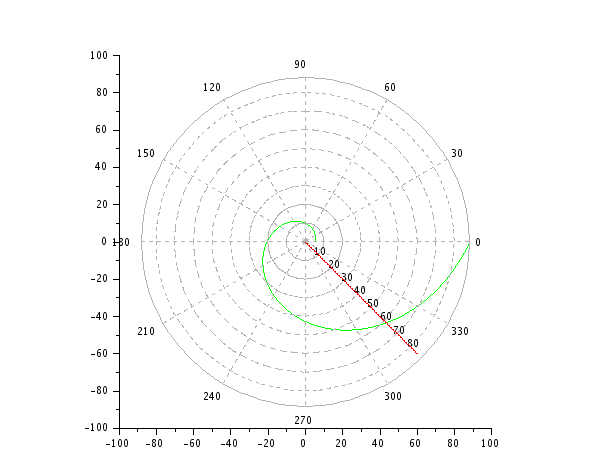
\includegraphics[width=\textwidth]{var2.png}\\
    \section{Точка пересечения}
    {\bf В первом случае}: $\theta = 315, r=25$\\
    {\bf Во втором случае}: $\theta = 315, r=60$
    
\end{document}s